\chapter[SCP-004 穿越锈钥之门]{
	SCP-004 The 12 Rusty Keys and the Door\\
	SCP-004 穿越锈钥之门
}

\label{chap:SCP-004}

\begin{figure}[H]
	\centering
	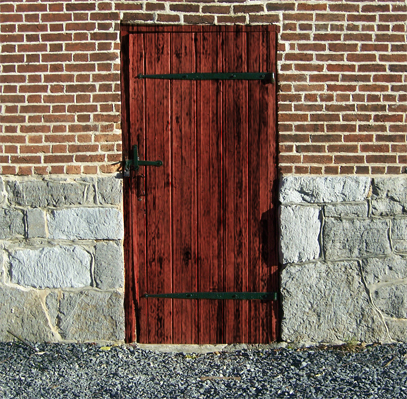
\includegraphics[width=0.5\linewidth]{images/SCP-004.jpg}
	\caption*{SCP-004-1}
\end{figure}

\bb{项目编号:}SCP-004

\bb{项目等级:}Euclid

\bb{特殊收容措施:}操作项目SCP-004-2至SCP-004-13时,严格遵守规程显得至关重要。只有在两名4级安保人员的陪同下,才允许将对象带离现场。严禁携带SCP-004的任何组分穿过SCP-004-1。该行为的后果尚不得而知,但其损失却将使深入的研究变成纸上谈兵。一旦SCP-004-1内部的对象脱离了管控,或设施遭到破坏,则必须赶在Site-62的导弹弹头激活之前将钥匙带回内部并给门上锁。未经授权而将钥匙移出试验区的行为足以成为就地处决的理由。

对SCP-004-1进行基本访问需1级许可;使用SCP-004-2至SCP-004-13需4级许可。

\bb{描述:}SCP-004包括一扇陈旧的木质仓库门(SCP-004-1)以及一组共计12把的生锈的金属钥匙(SCP-004-2至SCP-004-13)。门本身是位于【数据删除】的一座废弃工厂的入口。

\g{\bb{编年史}}

\bb{1949年7月2日}:三名少年非法侵入██████████附近联邦政府的房产时,发现了这扇门。根据证词,他们在一铁制保险箱内发现了一串生锈的钥匙,当即决定找出与钥匙对应的门。后来其中一人(SCP-004-CAS01)失踪,另外二人在联系司法长官█████████████████之后遭到了拘捕。

\bb{1949年7月3日:}地方当局在距SCP-004-1八公里处发现了SCP-004-CAS01被切断的右手,尸体的其它一些部分则四下散布,最远一处距厂区32公里。在讯问中,羁押的少年向当局坦白,当SCP-004-CAS01用其中一把钥匙开门时,身体突然被撕裂成若干碎片,可它们全都消失不见了。SCP基金会就此接管调查。

\bb{1949年7月4日:}SCP特工█████自地方当局处得到了钥匙以便开展试验,结果显示SCP-004-2至SCP-004-13全部适用于这扇紧闭的大门上的锁孔。12名D级人员被指定为受试者,持不同的钥匙进入房间以测试门的种种效应,结果仅有两人幸存,使用SCP-004-7及SCP-004-12以外的钥匙打开房门的受试者无一不被切割得七零八落。然而,直到后来才发现了肢解的尸块。撰写此记录时,只为每名受试者寻回两块尸块(使用SCP-004-█的受试者不在其列,此人的尸块零星散落在附近),其余皆杳不可寻。

两名幸存的受试者中,只有一人(使用了SCP-004-7)毫发无损。另一人则陷入了近乎紧张症的状态,踉跄地走到门口之后便瘫倒在地,且须随时看管起来,以防他抠出自己的双眼(见附录A:SCP-004-12对精神状态的影响)。使用SCP-004-7的受试者说他进入了一个巨大的空间,作为一栋附属的建筑来说未免大得离谱。在他撤离后,一个由3级人员组成的全副武装的小分队进入了强制开启的SCP-004-1,发现其空间的大小实在难以估量,门框和队员们是其中仅有的可以照亮和感知到的物体。

\bb{1949年7月16日:}处决了两名少年嫌犯及司法长官█████████████████。

\bb{1949年8月2日:}以“未引爆武器”为由宣布█████████████████为危险区,并在周边设立栅栏,防止平民进入。开始就暴露在SCP-004-1内部环境的安全性进行试验。

\bb{1950年12月1日:}已证实暴露在SCP-004环境下会引发时空异常。在另行通知之前,试验活动将暂停。

\bb{19██年7月2日:}一度下落不明的SCP-004-CAS01的残余部分意外地出现在SCP-004-1外部。虽然SCP-004-CAS01死于数十年前,尸体的残部却无丝毫腐败的迹象,且血不凝固,触感尚温。现已将其运走以进行相关测试。

\bb{19██年7月4日:}原12名受试者之一的失踪的残部以类似SCP-004-CAS01的方式重见天日。命名这部分尸体为SCP-004-CAS02。记录显示SCP-004-CAS01与SCP-004-CAS02均使用了SCP-004-██。

\bb{1999年3月21日:}鉴于核武器大规模扩散,距第三次世界大战仅余██年,在SCP-004-1内部某地启动了一项施工计划。该处用于储备足以供应███████人*天\footnote{\bb{译注:}人*天,统计单位,指每人每天完成的工作量,此处应用作每人每天消耗的物资。}的物资。

\bb{1999年4月21日:}█████████████████下令扩展SCP-004-1的内部站点,内容包括可以收容所有易于转移的SCP-███样本的应急仓库,以及可以存储全部SCP资料的██PB\footnote{\bb{译注:}1PB=1024TB,1TB=1024GB}的数据库。此处及其设施现称为Site-62。

\bb{2000年9月25日:}Site-62正式投入运作。实验室及管控单元全数就位,足以监管最危险的样本。SCP数据库的备份工作业已开始。

\bb{2001年1月25日:}由于时间的异常(见下文“时空异常”),现规定Site-62的全部工作人员必须永久居住在现场。已通知相关亲属其爱人在劳动事故中丧生,葬礼上的克隆尸体也预备妥当。

\bb{2003年7月14日:}美国东北部发生大规模停电,事故甚至波及到了加拿大。随着SCP的多个发电机接连失效,Site-62陷入了长达53分钟的停电中,伸手不见五指。现场人员报告说“觉察”到了某些人和生物,虽然当时并不能观察或感知到任何异样的实体。一些被选中的设施工作人员获准阅读████████████(附录A),他们表示“觉察”到的生物具有人类的体型,在某种程度上却与描述中的巨型绿色生物十分相似。

\g{\bb{时空异常}}

SCP-004似乎会传播时空异常,离开设施的人员纷纷报告遗失了时间。那些驻扎在站点数星期的人坚称只停留了几天,且作业记录和补给品的消耗量均可支持他们的论断。其它的时间异常则牵涉到SCP-004-2至SCP-004-13,尤其是SCP-004-CAS01和SCP-004-CAS02在使用过SCP-004-██后恰好██年时重新出现。现已委派████████████████████调查此类时间异常的方方面面。空间异常的例子则是通过SCP-004-7开启的那片广袤的区域,规模简直大得不可思议。同样,2003年的停电事故也表明,Site-62坐落的位置存在着一个交变的位面。

\g{\bb{详情注释}}

试验表明,钥匙中的10把都能将SCP-004-1开启为一个全新的维度,那里的构造和物理法则都与我们的世界大相径庭。遭遇如此险恶状况的受试者被大卸八块之后,尸块散落在不同的处所,经核实,只有三处是在地球。在其中的两处地点很快便发现了尸体,第三处地点的尸体则刚好出现在██年后的未来。其余七个地点尚不得而知。

目前的测试集中于两条研究途径:一是探寻在SCP-004的恶劣环境下生存的方法,二是【数据删除】主张SCP-004-2至SCP-004-13或许可以打开SCP-004-1之外的大门。

\g{\bb{附录A:SCP-004-12对精神状态的影响}}

所有使用SCP-004-12的D级人员归来时都陷入了紧张症状态,口不能言。其中一些保持足够体力的则不断试图挖出自己的双眼。16名受试者中共有4人幸存,仅有一人在长期心理治疗后恢复了对话能力,能够向精神科医生描述他所见的巨型绿色生物,巨大到其身体的大部分一直延伸至视野以外。他讲述着自己内心的惶恐,突然意识到它“好像已深深嵌入了(他)原初的恐惧之中”,并强行灌输着“无人能解”的记忆。受试者表现出严重的顺行性及逆行性遗忘\footnote{\bb{译注:}顺行性遗忘即无法记起患病之后的事件,逆行性遗忘即无法记起患病前的事件。}。

\g{\bb{附录B}}

\bb{项目编号:}SCP-004-14

\bb{发现日期:}1950年9月2日

\bb{对象来源:}发现于厂区的另一处地方——之前一直未发现的经纪人办公室。

\bb{描述:}该对象为一大型的质朴木箱,可以通过“安全”钥匙SCP-004-7开启,当然也可能是“危险”钥匙中的5把(见文档SCP-004-1)。

以SCP-004-7解锁SCP-004-14时,箱子通过铰链自行开启,其内部容量是同样容积在外部维度下容量的五倍。箱盖保持敞开状态,内部的物品对箱子的重量或其它属性无任何影响。然而当箱盖闭合并上锁后,所有物品与进入箱子的人员均消失得一干二净。然而以此方式消失的人员却似乎对【数据删除】的梦境产生了显著的影响。
